\subsection{HTTP Round Trip Times and Request Rates}
\label{subsec:rtt}

In that section the RTT time seen from different locations with a growing number of clients is presented. Furthermore the performance in requests per second is shown. The measurements are described by location ordered by a decreasing distance to the server

\subsubsection{Tokyo/Asia}

The measurements in Asia are performed with the highest base RTT of 280 ms. The graph in Figure \ref{fig:latency-asia}  represents the data for 4 measurements by using for each HTTP version two different pages (20kB, 1600kB). The number of clients is incremented by one  from 1 upto 750, while performing the measurements.

\begin{figure}[H]
	\centering
	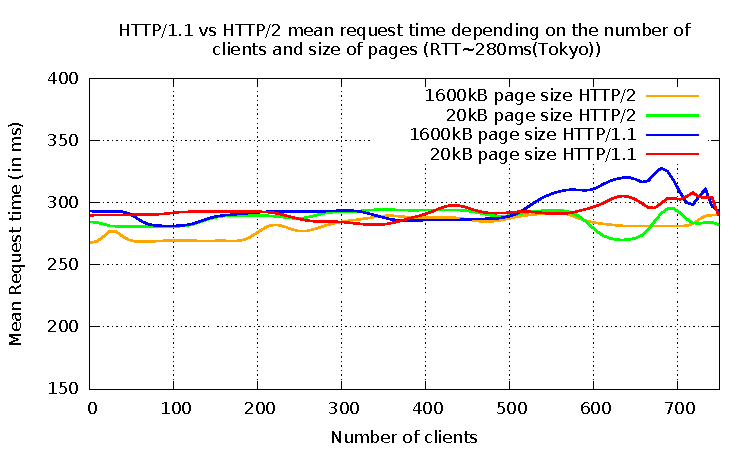
\includegraphics[scale=1,trim=0.0cm .0cm .0cm .0cm,clip]{images/latency-asia.pdf}
	\caption{Mean RTT measurements for Tokyo/Asia}
	\label{fig:latency-asia}
\end{figure}

A significant difference between both HTTP versions cannot be identified, although HTTP/2 is a few milliseconds faster during the measurements. The graph shows nearly a constant response time regardless if the number of clients increases. That can be explained by considering the rate of requests per seconds seen from the client in Tokyo. As more clients are added as more requests are being executed in approximately the same time. The graph in Figure \ref{fig:reqps-asia} shows that dependency.

\begin{figure}[H]
	\centering
	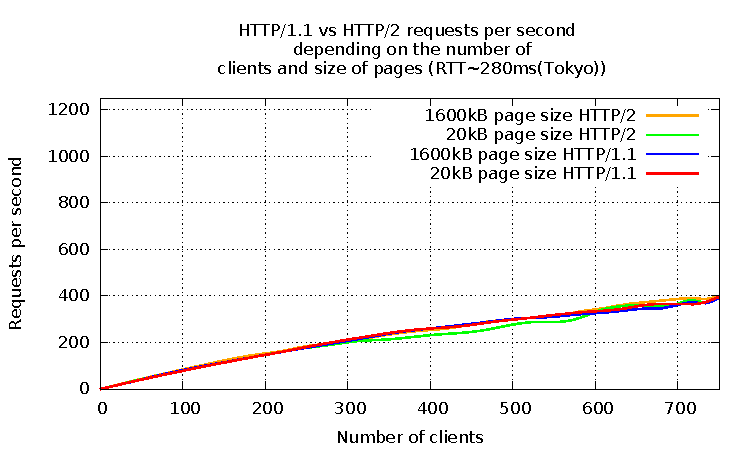
\includegraphics[scale=1,trim=0.0cm .0cm .0cm .0cm,clip]{images/reqps-asia.pdf}
	\caption{Mean Requests per second for Tokyo/Asia}
	\label{fig:reqps-asia}
\end{figure}

\subsubsection{North Carolina/North America}

The next measurements were taken from a client in North America/North Carolina with a measured base average RTT of 150ms and is shown in Figure \ref{fig:latency-na}. 

\begin{figure}[H]
	\centering
	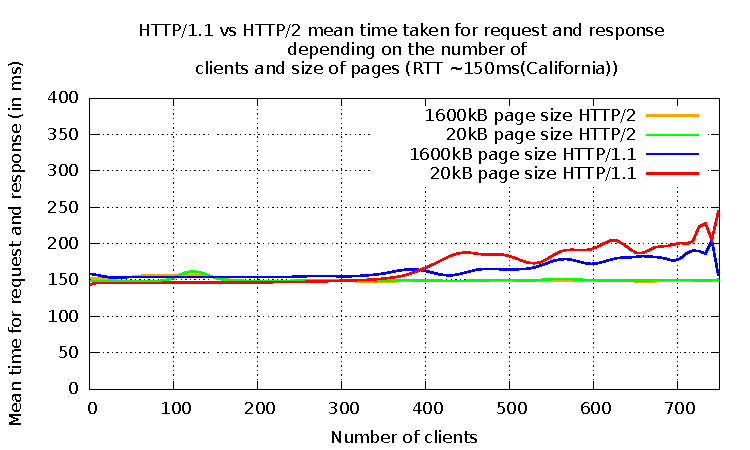
\includegraphics[scale=1,trim=0.0cm .0cm .0cm .0cm,clip]{images/latency-na.pdf}
	\caption{Mean RTT measurements for North Carolina/US}
	\label{fig:latency-na}
\end{figure}

The graph shows for HTTP/2 measurements, that the HTTP RTT is nearly almost equal to the measured base RTT. That means there is almost no jitter measurable and the RTT is constant for HTTP/2 requests regardless if the number of clients is raised or not. Moreover we see a growing HTTP/1.1 RTT starting from approximately 400 concurrent clients upwards. Figure \ref{fig:reqps-na} shows the corresponding request per second rate graph.

\begin{figure}[H]
	\centering
	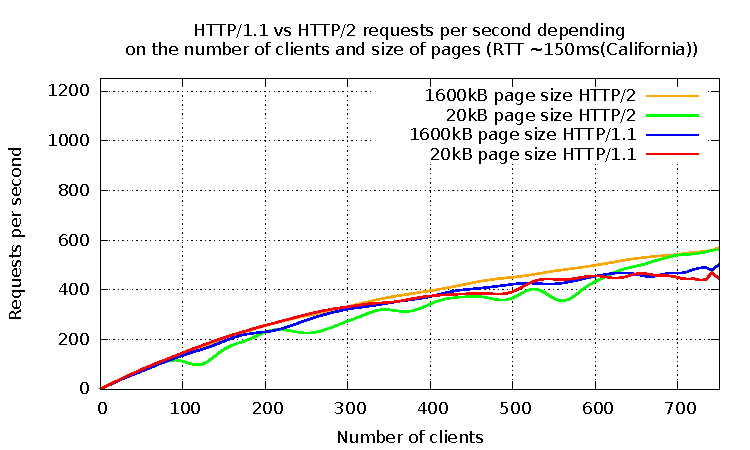
\includegraphics[scale=1,trim=0.0cm .0cm .0cm .0cm,clip]{images/reqps-na.pdf}
	\caption{Mean Requests per second for North Carolina/US}
	\label{fig:reqps-na}
\end{figure}

A slightly better request performance rate for HTTP/2 is the result of that mesurement. 

\subsubsection{Frankfurt am Main/Europe}

In contrast to the previous measurements, the measurements taken from a client in Frankfurt am Main/Europe are representing a low latency link with approximately 7ms of base RTT. The graph for the HTTP RTTs is shown in Figure \ref{fig:latency-europe}.

\begin{figure}[H]
	\centering
	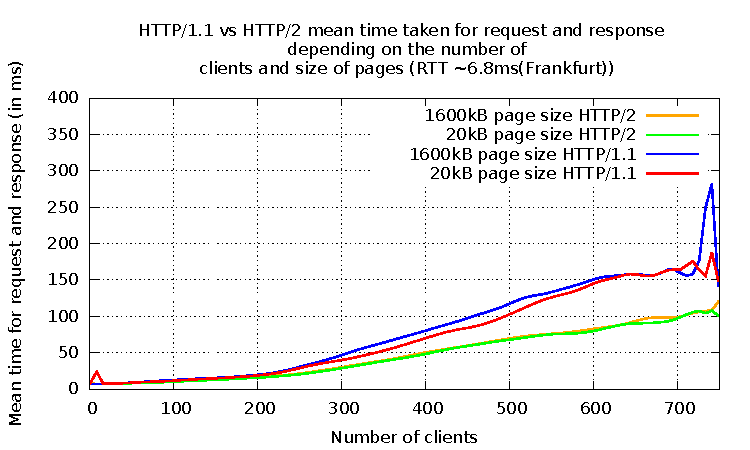
\includegraphics[scale=1,trim=0.0cm .0cm .0cm .0cm,clip]{images/latency-frankfurt.pdf}
	\caption{Mean RTT measurements for Frankfurt am Main/Europe}
	\label{fig:latency-europe}
\end{figure}

Compared to the previous measurements, the RTT graph looks different. Depending on the number of clients the RTT times grow nearly proportional. It is also a clear difference between HTTP/1.1 and HTTP/2 visible. The performed HTTP/2 measurements show significanltly less growing upto approximately 100ms for 750 clients, whereas the HTTP/1.1 RTT is for all measurements around 30\% slower ending up in a maximum of around 150ms. The  request rate graph shown in Figure \ref{fig:reqps-frankfurt} shows a different characteristic compared to the previous measurements.

\begin{figure}[H]
	\centering
	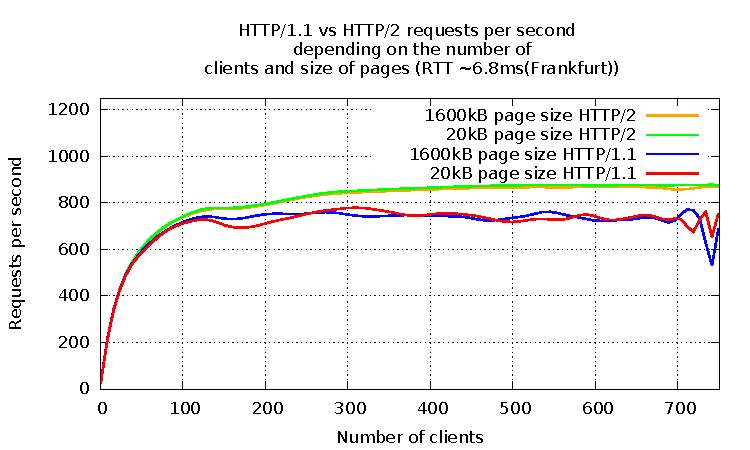
\includegraphics[scale=1,trim=0.0cm .0cm .0cm .0cm,clip]{images/reqps-frankfurt.pdf}
	\caption{Mean Requests per second for Frankfurt/Germany}
	\label{fig:reqps-frankfurt}
\end{figure}

It turns out that the request rate is identical to a asymptotic curve for all measurements. The server simply cannot handle more than approximately 800 concurrent connections. That is also the reason that after 100 concurrent concurrent clients the request rate remains nearly static. It is again visible that HTTP/2 performs better compared to HTTP/1.1. The fact that the base RTT for that measurement is significantly less than in the previous measurement, leads to much more connections at the same time at the server and different performance graphs.

\subsubsection{Amsterdam/Europe (local)}

Finally we performed measurements within the OS3 network (RTT 0.3 ms). We conducted those tests in two different ways. First we did separate measurements for each protocol version and then we conducted parallel tests in order to simulate workloads on the server for HTTP/1.1 and HTTP/2 requests simultaneous. Figure \ref{fig:latency-local} and Figure \ref{fig:reqps-local} show the graphs for the separate measurements.

\begin{figure}[H]
	\centering
	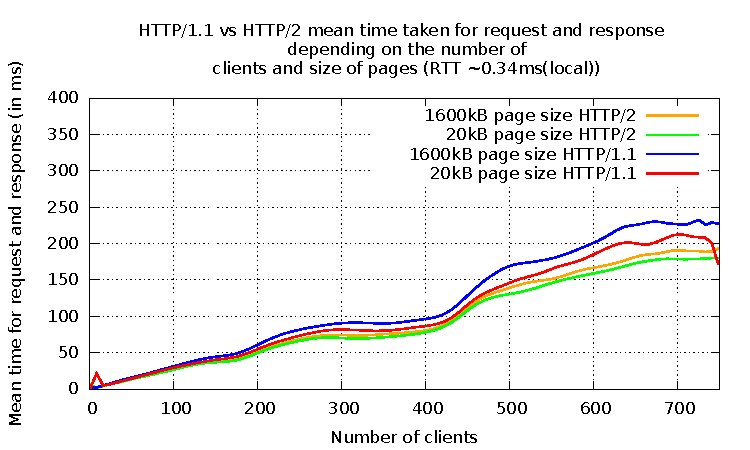
\includegraphics[scale=1,trim=0.0cm .0cm .0cm .0cm,clip]{images/latency-local.pdf}
	\caption{Mean RTT measurements for local/OS3 network}
	\label{fig:latency-local}
\end{figure}

\begin{figure}[H]
	\centering
	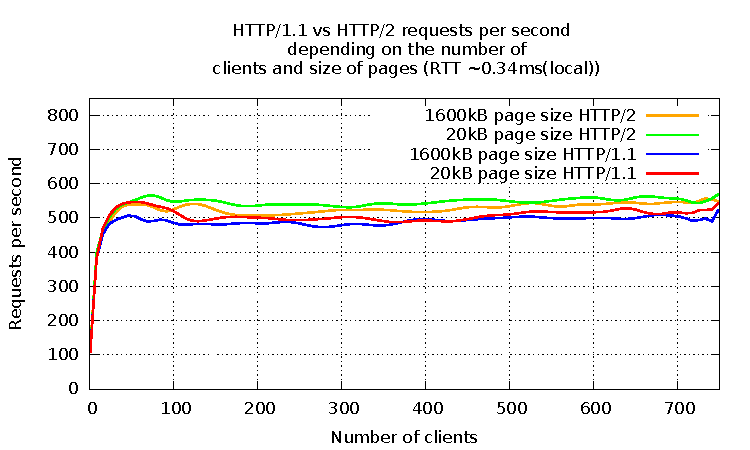
\includegraphics[scale=1,trim=0.0cm .0cm .0cm .0cm,clip]{images/reqps-local.pdf}
	\caption{Mean Requests per second for local/OS3 network}
	\label{fig:reqps-local}
\end{figure}

The graph characteristics is similar to the low latency link in Frankfurt. The difference between both measurements is the number of client needed to reach the server limit in terms or requests per second. The local measurement already reaches that limit at approximately 40 clients. That can be explained by the lower latency within the OS3 network resulting in a much faster connection establishment.
\\
\\
As a last measurement we conducted parallel tests for HTTP/1.1 and HTTP/2. The related graphs are shown in Figure \ref{fig:latency-localv1vsv2} and Figure \ref{fig:reqps-localv1vsv2}

\begin{figure}[H]
	\centering
	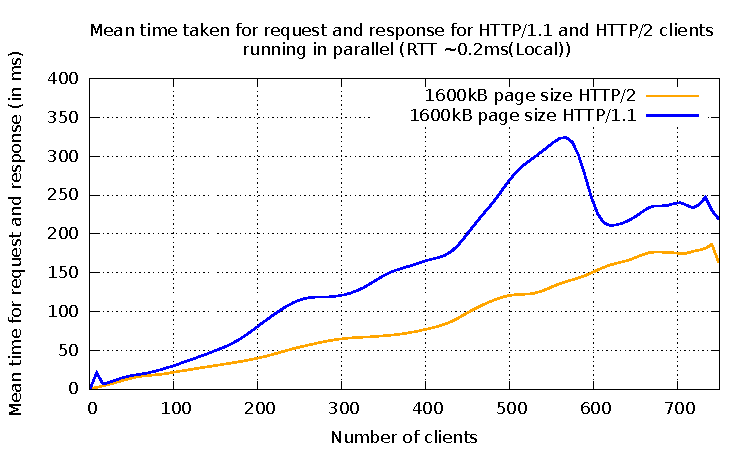
\includegraphics[scale=1,trim=0.0cm .0cm .0cm .0cm,clip]{images/latency-localv1vsv2.pdf}
	\caption{Mean RTT measurements for local parallel/OS3 network}
	\label{fig:latency-localv1vsv2}
\end{figure}

\begin{figure}[H]
	\centering
	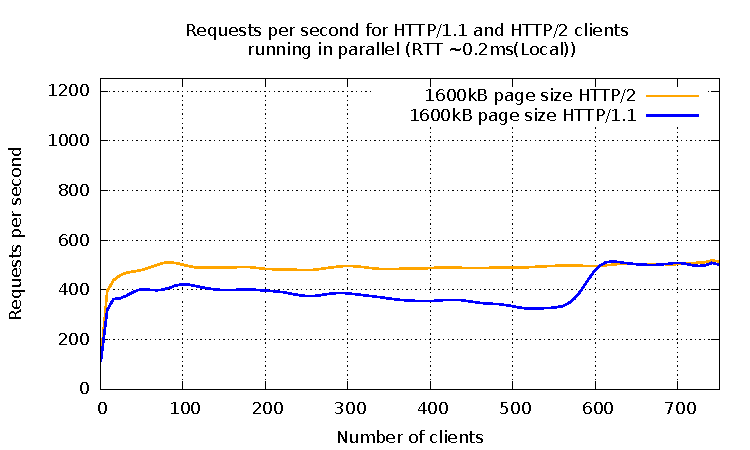
\includegraphics[scale=1,trim=0.0cm .0cm .0cm .0cm,clip]{images/reqps-localv1vsv2.pdf}
	\caption{Mean Requests per second for local parallel/OS3 network}
	\label{fig:reqps-localv1vsv2}
\end{figure}
 
The results of the local parallel measurements is showing again a significant difference between HTTP RTT times of both versions. HTTP/2 is clearly faster than HTTP/1.1. Figure \ref{fig:latency-localv1vsv2} shows a peak RTT for HTTP/1.1 at around 550 clients. At that moment the last HTTP/2 measurement was finished and afterwards the server was only busy with responding to HTTP/1.1 request. That is the reason for the decreasing RTT for HTTP/1.1 and the increasing number of requests per second starting  from that point.

\subsubsection{Mesurement analysis}

We can conclude that for almost all measurements the RTT time for HTTP/2 is significantly faster than for HTTP/1.1. That result is independent of the requested page size and also from the distance between client and server. For high latency links we discovered different characteristics regarding RTT and request rate compared to low latency links (Europe/Local). On low latency links (\textless 10ms) the number of requests per seconds grows much faster, which results in a quick saturation of the server to its maximum number of parallel requests. For high latency (Asia/North America) links a constant increase of RTT and request rate was measured for an increasing number of clients. In Figure \ref{fig:latency-all} all measured differences between HTTP/1.1 and HTTP/2 for all locations is shown. Lines above zero (y-axis) show a faster RTT for HTTP/2.

\begin{figure}[H]
	\centering
	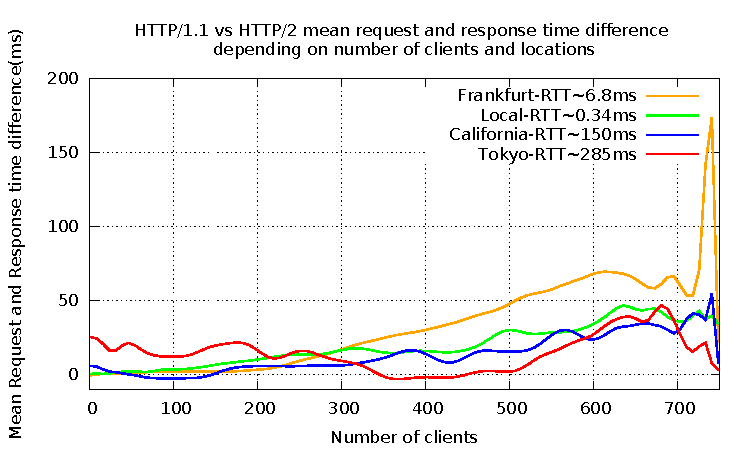
\includegraphics[scale=1,trim=0.0cm .0cm .0cm .0cm,clip]{images/difflatency.pdf}
	\caption{Mean RTT differences HTTP/1.1 - HTTP/2}
	\label{fig:latency-all}
\end{figure}

\newpage
